\chapter{Implementácia prostredia}
\begin{definicia}
Vlastné premenné robota sú premenné, ktorých adresu pozná len robot a tak nie je možné s nimi manipulovať od inakiaľ ako z vnútra robota.
\end{definicia}

Každý robot má vlastný program, užívateľom definovaný, podľa ktorého sa správa. Tento program sa z hľadiska jednotlivého robota skladá z postupnosti základných inštrukcií (detailnejšie vysvetlené nižšie). Pre plynulosť simulácie je potrebné zaistiť spravodlivosť pri vykonávaní programu, v opdstate ide o zahovanie zdania simultánnosti robotov. Ako bolo povedane skôr Robot totiž môže počítať s vlastnými premennými, na ktoré nepotrebuje dáta bojiska, teda nemusí na nič čakať. Zaistenie spravodlivosti v tomto prípade teda znamená,  oby o Toto je splnené tým, že každá inštrukcia je penalizovaná, preto sa najskôr budeme zaoberať penalizáciou a nie samotným priebehom.
\section{Priebeh penalizácie za inštrukciu}

\begin{definicia}
Tick je jednotka virtuálneho času sveta. 
\end{definicia}

\begin{definicia}
Penalizáciou za inštrukciu nazývam počet tikov, ktoré robot stratí, ak inštrukciu vykoná. Pre rôzne inštrukcie môže byť rôzna.
\end{definicia}

\begin{definicia}
Programom robota sa nazýva postupnosť inštrukcií, ProgramPointer je ukazateľ na inštrukciu v programe. Druhy inštrukcií a ich vplyv na svet je popísay v \ref{TODO}.
\end{definicia}

Nech je na rade robot R. V tomto okamihu začne R vykonávať inštrukciu, na ktorý práve ukazuje jeho ProgramPointer. Ako je naznačené na \ref{thinking}, robot pokračuje vo vykonávaní inštrukcií až kým nenarazí na takú, ktorá interaguje s bojiskom. Výsledok takejto inštrukcie nie je možné zistiť z dostupných informácií a teda je nutné o ďalšie data požiadať bojisko. Podľa veľkosti penalizovania sa potom R zaradí do plánovaných objektov, viz \ref{timeline}. Dĺžka tejto akcie sa ale pre rovnaký počet inštrukcií pre dvoch rôznych botov môže a typicky bude líšiť. Je to spôsobené tým, že každá inštrukcia môže mať rozdielnu penalizáciu za vykonanie. Napríklad samostatné vykonanie inštrukcie 'step' musí byť niekoľko krát rýchlejšie ako povedzme inštrukcia, ktorá naloaduje hodnotu premennej, obzvlášť ak táto premenná už dlho loadovaná nebola. Ďalej inštrukcia, ktorá zavolá užívateľom definovanú funkciu, zaberie viac procerového času vzhladom na to, čo musí spraviť so zásobníkom robota, a preto je táto skutočnosť zohľadnená. Podobne napríklad inštrukcie pre násobenie a delenie su zlošitejšie ako prosté sčitanie a preto sú viac penalizované. Penalizácia prebieha podľa tabuľky \ref{penal}, je možné si ale v nastaveniach nastavit tieto funkcie:
\begin{itemize}
\item SizeOfFunction: počet inštrukcií vo funkcii
\item SizeOfCleaned: počet premených, ktoré sa stali odchodom z bloku príkazov neplatnými. Použiteľné iba pri inštrukcii indikujúcej koniec bloku
\item LastLoaded: počet tickov, ktoré ubehli od posledného loadovania premennej alebo funkcie, použiteľná iba s inštrukciami Load a Call
\end{itemize}
\begin{table}[ht]
\centering
\caption{Výpočet penalizácie inštrukcie}
\begin{tabular}{|c | c |}
\hline
Inštrukcia & Penalizácia \\
\hline
Jump & 0\\
Store & 1 \\
Plus & 1 \\
Minus & 1 \\
Multiply & 2 \\
Divide & 4 \\
Less & 1 \\
LessEqual & 2 \\ %kontroluje sa aj real/integer!
Call &  0 \\
StartBlock & 0 \\ %iba zvysi aktuane zanorenie
EndBlock &  SizeOfCleaned \\
Load & 1\\
Return & 1 \\
Restore & 1 \\
\hline
step & 1\\
see & 3\\
shoot & 1\\
turn & 1\\ 
turnL & 1\\
turnR & 1\\
\hline
\end {tabular}
\label{penal}
\end{table}

\begin{figure}
\centering
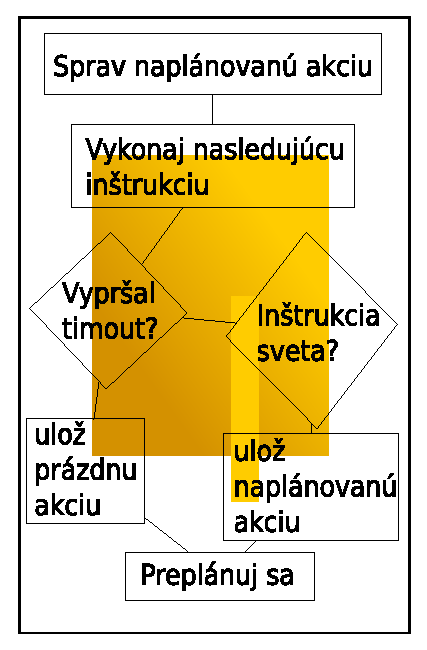
\includegraphics[totalheight=0.2\textheight,width=.2\textwidth]{thinking}
\caption {Priebeh premýšľania u robota}
\label{thinking}
\end{figure}

Robotovi môže týmto spôsobom samozrejme vypršať čas, veľkosť jeho premýšľania dosiahne hodnoty timeout.%TODO ref
V takom prípade, ako je naznačené na obrázku \ref{thinking} sa robot vzdá, preplánuje sa a uvoľní miesto nasledujúcemu objektu. 
\newline
Nech je na rade objekt rôzny of typu 'robot'. Potom tento objekt má konštantnú penalizáciu a jeho program obsahuje iba inštrukcie, ktoré interagujú s bojiskom.Sú rôzne v závislosti na type objektu.

\subsection{Preplánovanie}

Preplánovanie prebieha tým spôsobom, že sa podľa tabuľky \ref{penal} spočíta, koľko času robot prehmrhal na myslenie, presne o toľko sa posunie v pomyselnej casovej osi a zaradí sa vo fronte udalostí za posledného bota s rovnakým časom. To spôsobí to, že robot, ktorý nebol na rade dlhšie, sa dostane k akcií skôr, čo je opäť jedna z podmienok fair-play.\\
V tomto prípade sa za kľúč, podľa ktorého sa objekty usporadúvajú, považuje čas od začiatku behu hry. Problém ale nastáva v okamihu, keď tento čas pretečie. Vzhľadom na to, že celkový čas simulácie je ukladaný do 64-bitového integeru, je možnosť, že by tento čas pretiekol, krajne neprijateľný, pretože celkový čas by bol vačší ako niekoľko tisíc rokov:)\\
Otázkou zostáva, ako implementovať túto časovú líniu tak, aby celý program nepůsobil trhane, teda aby v okamihu, keď robot rozmýšľa, ostatné objekty, ktoré sú na rade, sa mohli pohybova+t, keďže samotné premýšľanie sa ich nedotýka. Existuje niekoľko možností:
\begin{itemize}
\item Z robotovho programu sa približne odhadne, koľko budei minimálne premýšlať a po tomto čase sa pozrie, či výpočet dobehol. Ak nie, bude musieť čakať, ak áno, pokračuje sa s zozbrazovaním akcií, ktoré sú výsledkom inštrukcií objektov. 
Výhody tohoto prístupu:\begin{itemize}
	\item Plus: Je zachovaná správna postupnosť akcií, to znamená, že nie sú závislé na procesore a jeho súčasnej vyťaženosti.
	\item Minus: Odhad sa můze od skutočnej penalizácie líšiť stovky tickov (napríklad v prípade u podmieneného skoku sa načíta funkcia, ktorá stoji ohromne moc, kým v druhej vetve sa robot okamžite pohne), tým by vznikali nechcené prestoje a simulácia by sa v istých situáciách trhala.
	\end{itemize}
\item Dopredu sa nasimuluje časť priebeh hry a na výstup sa púšťajú už iba výsledky. Výhody a nevýhody:
	\begin{itemize}
	\item Plus: Simulácia sa bude zatrhávať maximálne raz za čas, v okamihu, keď ešte nebudú pripravné data, čo sa 
	\item Minus: na jednoprocesorovych architekturach ma tento spôsob rovnaký efekt ako keď sa súčasne vykresľujú oneskorené výsledky a súčasne poćítajú aktuálne časové línie.
	\end{itemize}
\end{itemize}
Kód robota sa za jeho života nemení. 

\section{Hracia plocha} % z coho sa sklada
Na začiatku hry sa vygeneruje mapa s veľkosťou, ktorú zadá užívateľ, alebo sa načíta už uložená mapa. Táto pozostáva zo voľných políčok a stien. Steny sú rôzneho typu, viz \ref{kap}. Ďalej celú túto konštrukciu nazývam bojisko. V tomto okamihu je hra pripravená na spustenie. V závislosti na veľkosti bojiska sa čaká na odpovedajúce množštvo robotov, ktorí sa zapoja do hry. Toto množstvo je defaultne obmedzené iba zdola. Na zdôvodnenie tohoto rozhodnutia je nutné spomenúť základné vlastnosti programu. 
garantovaný, nastávajú dve možnosti, ako to tom informovať robota:
\begin{itemize}
\item za cieľ by sa simulovalo ľubovoľné políčko, ktoré je mimo mapy. V tomto prípade by robot prinajlepšom cyklicky prehľadával celú mapu, čo je v podstate to isté akoby pozíciu vôbec nepoznal.
\item za cieľ by sa vybralo políčko patriace mape. V tom prípade 
\item Je zabezpečená spravodlivosť pre robotov. To znamená
\end{itemize}

v  že pri neprimarane veľkých mapách bude trvať príliš dlho, než sa roboti vobec  
Nastavenie toho, ze roboti so takto obmedzení, a dá prenastaviť v settings.%TODO rozpisat v+setky menu, +co kde robia
\subsection{Generovanie map}% ako sa generuje, podpora ukladania, zadne zhluky, vyhody, nevyhody, 
\section{Jazyk hry a priebeh hry} %bison, preco
\begin{definicia}
Cieľom určenia robota nazývam políčko na mape sveta, kam sa má robot dostať. Teda ak je pozícia robota rovnaká ako pozícia tohoto cieľu, hra končí. Týchto cieľov môže byť viac. V prípade viacerých cieľových oblastí má užívateľ možnosť zvoliť voľbu \it{Vlastný Exit}, kde sa každému robotomi priradí práve jedna cieľová pozícia a to tá najvzdialenesia od jeho výskytu v mape po začatí hry.
Pod vzdialenosťou rozumiem veľkosť obsahu obdĺžnika v vrcholmi cieľom a výskytom robota. %TODO preco?
\end{definicia}

Samotná hra prebieha tak, že roboti vykonávajú užívateľom definovaný kód až do okamžiku, keď dosiahnu cieľ určenia alebo kým zostane na bojisku maximálne jeden robot. Cieľ môže byť pre každého robota rozdielny a je súčasťou mapy sveta. Hra nie je zabezpečená proti nekonečne dlhotrvajúcim cyklom (napríklad keď každý robot stojí na mieste), predpokladá sa v tomto prípade vstup od uživateľa, ktorým hru prerusí.

\begin{definicia}
Stav robota vzhľadom na svet charakterizuje štvorica: (InstructionPointer IP, Hitpoints HP, VisualMemory vm, Direction direct), kde 
\begin{itemize}
\item InstructionPointer je odkaz do štruktúry programu robota hovoriaci, ktorá inštrukcia je na rade
\item HP je nezáporné celé číslo popisujúce životnosť robota
\item VirtualMemory je štruktúra obsahujúca objekty v zornom poli od posledného volania funkcie 'see()', volanej bez parametrov 
\end{itemize}
Stav robota s ohľadom na inštrukcie, ktore vykonáva, charakterizuje (PointerStack PS, ValueStack VS, Memory m) kde
\begin{itemize}
\item PS zoznam pointerov do štruktúry programu
\item VS je zásobník všetkých naloadovaných hodnôt, parametrov  a návratových adries z funkcií
\item Memory je zoznam všetký doteraz definovaných premenných a funkcií
\end{itemize}
\label{StavRobota}
\end{definicia}

\begin{definicia} 
Pod objektami sveta rozumieme všetky prvky, ktoré svet tvoria a zároveň ho z času na čas menia, t.j. v tomto prípade strely, steny, a samotní roboti. Napríklad strela mení svet tým, že sa pohne alebo narazí, istý druh steny sa môže posunúť a pod.
\end{definicia}
Svet je charakterizovaný dvojicou $< FrontaUdalosti, Bojisko >$, kde FrontaUdalosti je fronta objektov, ktoré sú na rade, aby komunikovali so svetom. Presný spôsob definovania poradia tejto komunikácie je popísaný neskôr. Objekty v tejto fronte sa počas priebehu boja menia, napríklad pribúdajú a zanikajú strely, ktoré sú podla \ref{defobjekty} tiež objektami.

Pre všetky nasledujúc inštrukcie interagujúce so svetom predpokladajme, že svet je v stave $<FrontaUdalosti, Bojisko>$, kde FrontaUdalostí je postupnosť objektov $(robot X, objekt1, objekt2, objekt3,...objektN)$ a Bojisko je dvojrozmerná matica popisujúca, aké objekty sú na akých pozíciach.
Popis jednotlivých inštrukcií a ich vplyv na svet je symbolicky popísaný takto: (bez parameterov, ktoré nemajú vplyv na svet):\\
\newline
step:\begin {itemize}
\item Svet:$ < NewQueue, m.reinsert(X) > $
\item Bot: $ < NewIP, HP, direct> $
\end {itemize}
turnLeft, turnRight \begin{itemize}
\item $Svet:  <NewQueue, m>$
\item $Bot:  < NewIP, Hp, NewDirect)>$
\end{itemize}
turn  \begin{itemize}
\item $Svet:  < NewQueue, m > $
\item $Bot:   < NewIP, Hp, NewDirect)> $
\end {itemize}
see  \begin{itemize}
\item $Svet:  <NewQueue,m> $
\item $ Bot:  < NewIP, Hp, NewDirect)> $
\end {itemize}
shoot \begin {itemize}
\item $ Svet:  < AddQueue, m> $ 
\item $ Bot:  < NewIP, Hp, Direct)>  $
\end {itemize}
\indent
kde NewQueue je \\ $(Objekt_1, Objekt_2, ..., Objekt_K, X, Objekt_{k+1},.., Objekt_N)$, NewIP je nový ukazateľ do programu robota, nie nutn odlišný od predošlého, NewDirect je číslo 1-4 označujúce aktuálne natočenie robota, reinsert je funkcia, ktorá sa pokúsi robotom pohnut v mape, ak sa nedá vyvolá sa ošetrenie kolízií a AddQueue je\\ $(Objekt_1, Objekt_2, ...,Object_{strela},..., Objekt_K, X, Objekt_{k+1},.., Objekt_N)$ (strela bude na rade typicky pred robotom, ktorý j vypustil, pretože ten robot sa preplánuje, ale strela ešte na rade nebola, tak mś vyššiu prioritu.)
Ďalšie inštrukcie vôbec nekomunikujú so svetom, preto sú uvedené oddelene. Tieto inštrukcie robot vykonáva počas svojho premýšľania. Keďze tým robot vobec nepotrebuje vedieť o objektov sveta iných než je on sám, po prevedení takýchto inštrukcií sa meni stav robota podla tabuľky \ref{VnutroBota},kde IP+1 znamená posun v atuálneho pointera v programe robota o jednu inštrukciu ďalej, AddedIP je uloženie aktuálneho pointera na inštrukciu a vyhlásenie iného pointera za aktuálny (typicky začiatok pricedúry alebo funkcie), VariablesAdded je pamať robota rozrastená o premenné danej funkcie alebo procedúry v danom zanorení, ClearVariables je označenie premennych definovaných v tomto bloku za neplatné, LoadByName je uloženie hodnoty volanej premennej na ValueStack, AddedResult je uloženie výsledku aritmetických operácií na ValueStack a DeleteIP je zrušenie aktuálneho pointera na funkciu a obnovenie predchádzajúceho na inštrukiu, pre ktrou bol prerušený. RemoveValue je spracovanie hodnoty zo ValueStacku a teda jej odobranie a odobranie premennej, do ktorej sa priradzuje.

\begin{table}[ht]
\centering
\caption{Vnutorné príkazy robota}
\begin{tabular}{|l|p{5cm}|}
\hline\hline
Inštrukcia & Stav bota po inštrukcii \\
store & $ IP+1,RemoveParameters$\\
aritmeticke+relacne operácie & $IP+1,AddedResult,m$ \\
Call &  $ AddedIP,VS,VariablesAdded$\\
StartBlock & $IP+1,VS,m$\\
EndBlock & $IP+1,VS,ClearVariables$\\
Load & $ IP+1,LoadByName,m$\\
Label & $ IP+1,VS,m$\\
Jump & $ DeleteIP,VS,t$\\
\hline
\end{tabular}
\label{VnutroBota}
\end{table}

\subsection{Zrak robota}
V úvode si užívateľ má možnost nastavit dve premenné, ktoré ovplyvňujú to, ako ďaleko bude robot vidieť. Sú to premenné X, Y, ktoré označujú obdĺžnik, podľa ktorého sa zrak ďalej určí.

\begin{figure}
\centering
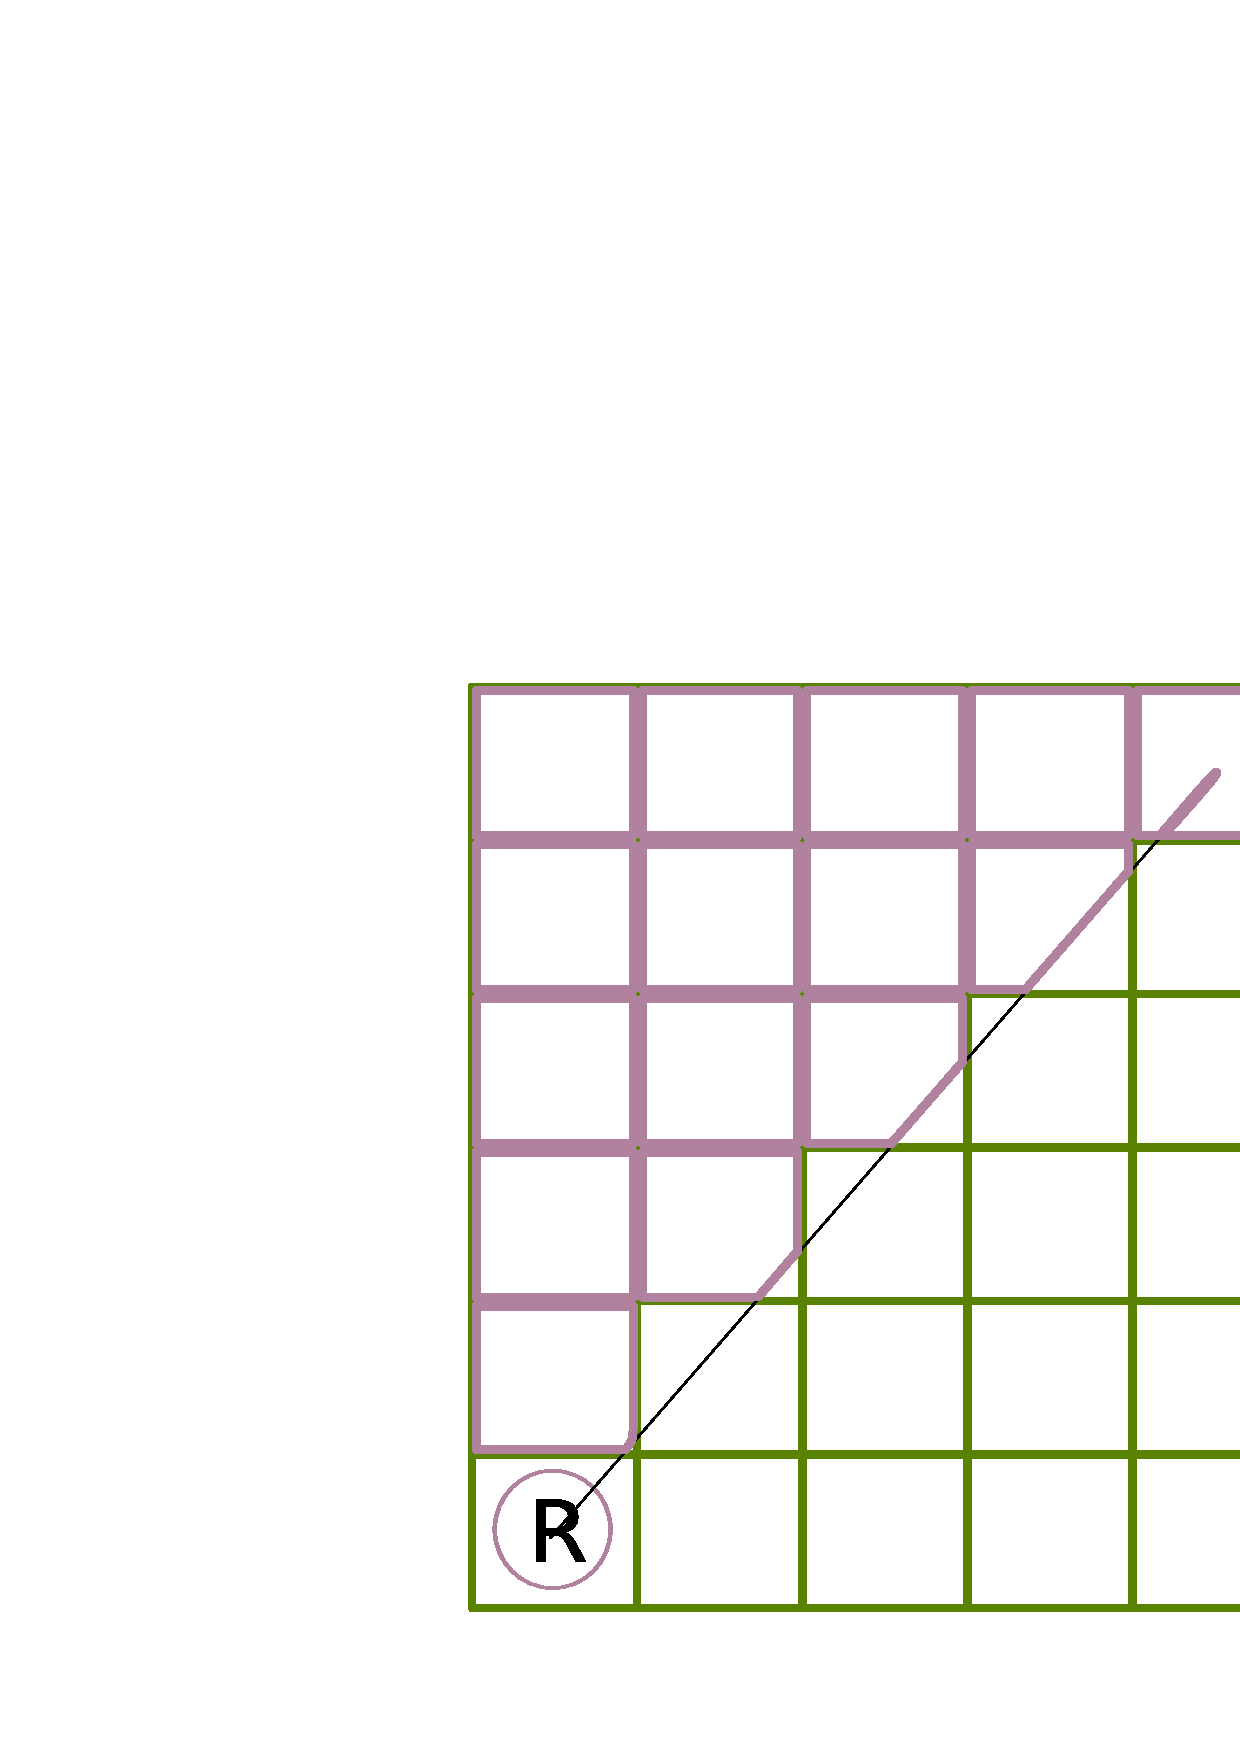
\includegraphics[totalheight=0.2\textheight,width=.6\textwidth]{chooseVisible}
\caption {Výber parametrov pre zrak robota}
\label{choosing}
\end{figure}

\begin{definicia}
Pod zorným poľom robota rozumieme hornú polovicu trojuholníka určeného uhlopriečkou medzi vrcholmi obdĺžnika o veľkosti X,Y. Robot vidí objekt v okamihu, ked vidí stred políčka, na ktorom objekt stojí a úsečka spájajúca tieto dva body nepretína žiadny ďalší blokujúci objekt. blokujúci objekt je definovaný implementáciou, v našom prípade je blokujúci objekt robot a stena, neblokujúci strela. toto rozdelenie vychádza z bežneho pozorovania, že drobná stela nemá tendenciu zakrývať výhľad.
\end{definicia}
Obdĺžnik môže mať vzhľadom na implementáciu maximálne obsah 32, čo je na väčšine architektúrách veľkosť integeru. Toto číslo bolo zvolené, pretože je dostatočne veľké a súčasne vysoko dostupné na rôznych architektúrach. Samotne detekovanie toho, čo robot vidí, prebieha nasledujúco: \\
\begin{figure}
\centering
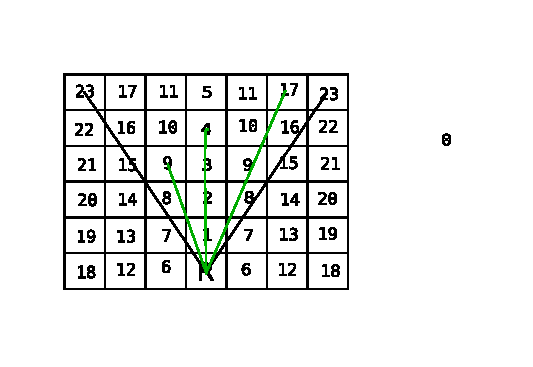
\includegraphics[totalheight=0.4\textheight,width=.8\textwidth]{visibility}
\caption {Viditeľnosť robota s parametrami x = 5, y = 6}
\label{visibility}
\end{figure}
Nech má obdĺžnik rozmery (x,y) a jeho dolný ľavý vrchol je na pozícií (0,0), čo je v podstate pozícia bota. Obdĺžnik je teda rozdelený na XxY menších obdĺžničkov. Kazdý z nich má svoje poradové číslo a masku, ktorá má na i-tej pozícií jedničku práve vtedy, ak úsećka počínajúca v bode [0.5,0.5],čo je stred políčko s robotom, a stredom skúmaného políčka prechádza políčkom s identifikaćným číslom ID. takto ale robot bude vidieť len na jednu stranu, ale keďže druhá polovička je presne symetrická, môžeme tieto práve vygenerované masky použiť, viz \ref{visibility}  na obe strany bez upravovania. \\
Podla obrázka \ref{visibility} bude mať políčko s ID 4 masku 1111, pretože na to, aby ho bolo vidno, je nutné vidieť políčka s ID 1,2,3. Podobne políčko 9 bude mať masku 110000011, pretože úsečka spájajúca tieto dva body prebieha tiež týmito políčkami. Zistenie, či práve toto políčko je pretnuté úsečkou, sa takto zjednodušuje na nájdenie všeobecnej rovnice priamky s koncovými bodmi v stredoch týchto dvoch políčoka zistenie, či pravý dolný vrchol a ľavý horný vrchol patria rovnakej polrovine generovanej touto priamkou.\\

Za života robota sa jeho zrak nemení a teda môžeme použiť tieto vygenerované masky bez ďalšieho prepočítavania. Pri volaní metody see(), ktorá dodá viditeľné objekty robotovi, potom stačí namapovať náš obdĺžnik na príslušné miesto na mape(podľa robotovej pozície a natočenia), nastaviť 1 na i-té miesto políčka s ID = i, na ktorom nie je nič alebo len neblokujúci objekt, a výslednú masku porovnať s predtým vypočítanou maskou každého políčka, na ktoré by robot mohol vidieť. Nech zisťujeme, či vidíme objekt na pozícií na mape X,Y, ktorý sme namapovali na políčko s ID = I a maskou M. Ak výsledná maska má jedničky presne na tých istých miestach ako M, potom I je viditeľné, pretože všetky políčka, na ktorých I záviselo, boli označené ako viditeľné. \\
Nech existuje také políčko s ID = P, na ktorom je nejaký blokujúci objekt. Potom vo výslednej maske bude na P-tom mieste 0 a políčko I, ak úsečka spájajúca stredy políčok robota a I prechádzala cez P, bude mať na P-tom mieste 1. Maska políčka I bude mať teda o minimálne jednu 1 viac ako výsledná maska a teda políčko bude označené ako neviditeľné.\\
Na obrázku \ref{visibleo} je červeným znázornen=y objekt, ktorý robot uź neuvidía zelenou, ktorý uvidí. Napríklad je viditeľný robot R, pretože pred ním je strela S a keďže je neblokujúca, políčko 4 pripojilo na výslednej maske 1 na 4.pozícií. Pozícia 5 má masku 1111 a teda je viditeľná.

\begin{figure}
\centering
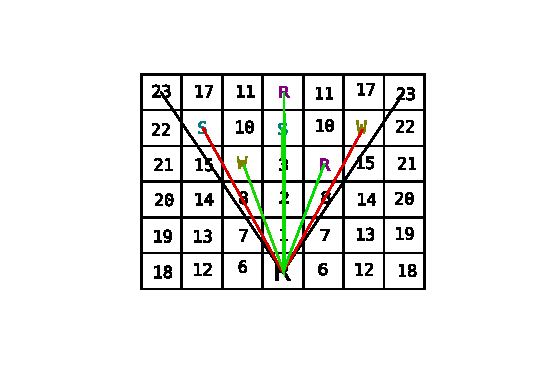
\includegraphics[totalheight=0.4\textheight,width=.8\textwidth]{VisibleObjects}
\caption { Objekty v zornom poli robota}
\label{visibleo}
\end{figure}
\indent

\subsection{Priebeh výpočtu robota} %co je povolene a ako sa to riesi implementacne
..\\
Zaujímavejšie je to pri volaní funkcie, ktorá má defaultný parameter. Pretože sa predpokladá, že program bude prístupný aj pre obyčaných užívateľov, je možné u funkcie definovať aj explicitnú hodnotu a to nezávisle na poradí parametrov. T.j. explicitné hodnota môže byť zadaná ako prvý a tretí parameter, ale nie ako druhý. Takáto funkcia sa nadefinuje podobne ako v C/C++, napríklad : \\\center $ function distance(integer x=3, integer y=2, integer radius, Location l) $ \\ je funkcia, ktorá bude napr
\subsection{Detekcia zacyklenia}

Užívateľ si typ strely definuje tak, že dostane k dispozícií určitź počet bodv a tie musí medzi jednotlive volby rozdeliť\\
Bot premýšla tak, že sa nechá bežat dovtedy, kým z jeho program nenarazí na inštrukciu, ktorá by ovplyvnila svet, alebo kým neprsiahne timeout. Ak presiahne timeout, preruší sa, preplánuje vo fronte udalostí ďalej (presnejšie o TIMEOUT tikov ďalej)\\
Velmi špeciálny je prípad, keď užívateľ nenastaví robotovi žiadnu pamať. Takýto robot nie je schopný si zapatať jedinú premennú a ani vracat návratové hodnoty, teda v kóde programu by nemali byť definované žiadne funkcie, ale iba procedúry.Je nutné povedať, že funkcie a procedúry sa v žiadnom prípade nechovajú ako premenné a teda nezaberajú robotovi pamať. Teda v tomto prípade dojde k masívnemu využitiu rekurzií. Samotne vstavané príkazy sú však vlastne funkcie, ale kedže sa nikam nemajú priradiť, ich návratová hodnota sa zahodí. Nevýhodou tohoto typu bota je však skutočnost, že nemá povolené napriklad strieľanie, pretože to je funkcia, ktorá potrebuje za každých okolností parametre.
